% !Mode:: "TeX:UTF-8"
\chapter{Lie Group and Lie Algebra}
\label{cpt:4}
\begin{mdframed}
    \textbf{Goal of Study}
    \begin{enumerate}
        \item Learn the concept of Lie group, Lie algebra, and their applications of $ \mathrm{SO}( 3 ), \mathrm{SE}( 3 ) $ and the corresponding Lie algebras.
        \item Learn the meaning and usage of the BCH (Baker-Campbell-Hausdorff) formula.
        \item Learn the perturbation model on Lie algebra.
        \item Use Sophus to perform operations on Lie algebras.
    \end{enumerate}
\end{mdframed}

In the last lecture, we introduced the description of rigid body motion in the three-dimensional world, including the rotation matrix, rotation vector, Euler angle, quaternion, and so on. We focused on the representation of rotation, but in SLAM, we have to estimate and optimize them in addition to the representation. Because the pose is unknown in SLAM, we need to solve the problem of which camera pose best matches the current observation. A typical way is to build it into an optimization problem, solving the optimal $ \mathbf{R}, \mathbf{t}$ and minimizing the error.

As mentioned before, the rotation matrix itself is a constrained (orthogonal, and the determinant is 1) matrix. When used as optimization variables, it introduces additional constraints on matrices that make optimization difficult. Through the transformation relationship between Lie group and Lie algebra, we can turn the pose estimation into an unconstrained optimization problem and simplify the solution. Considering that the reader may not have the basic knowledge of Lie Group and Lie algebra, we will start with the most basic knowledge.

\newpage
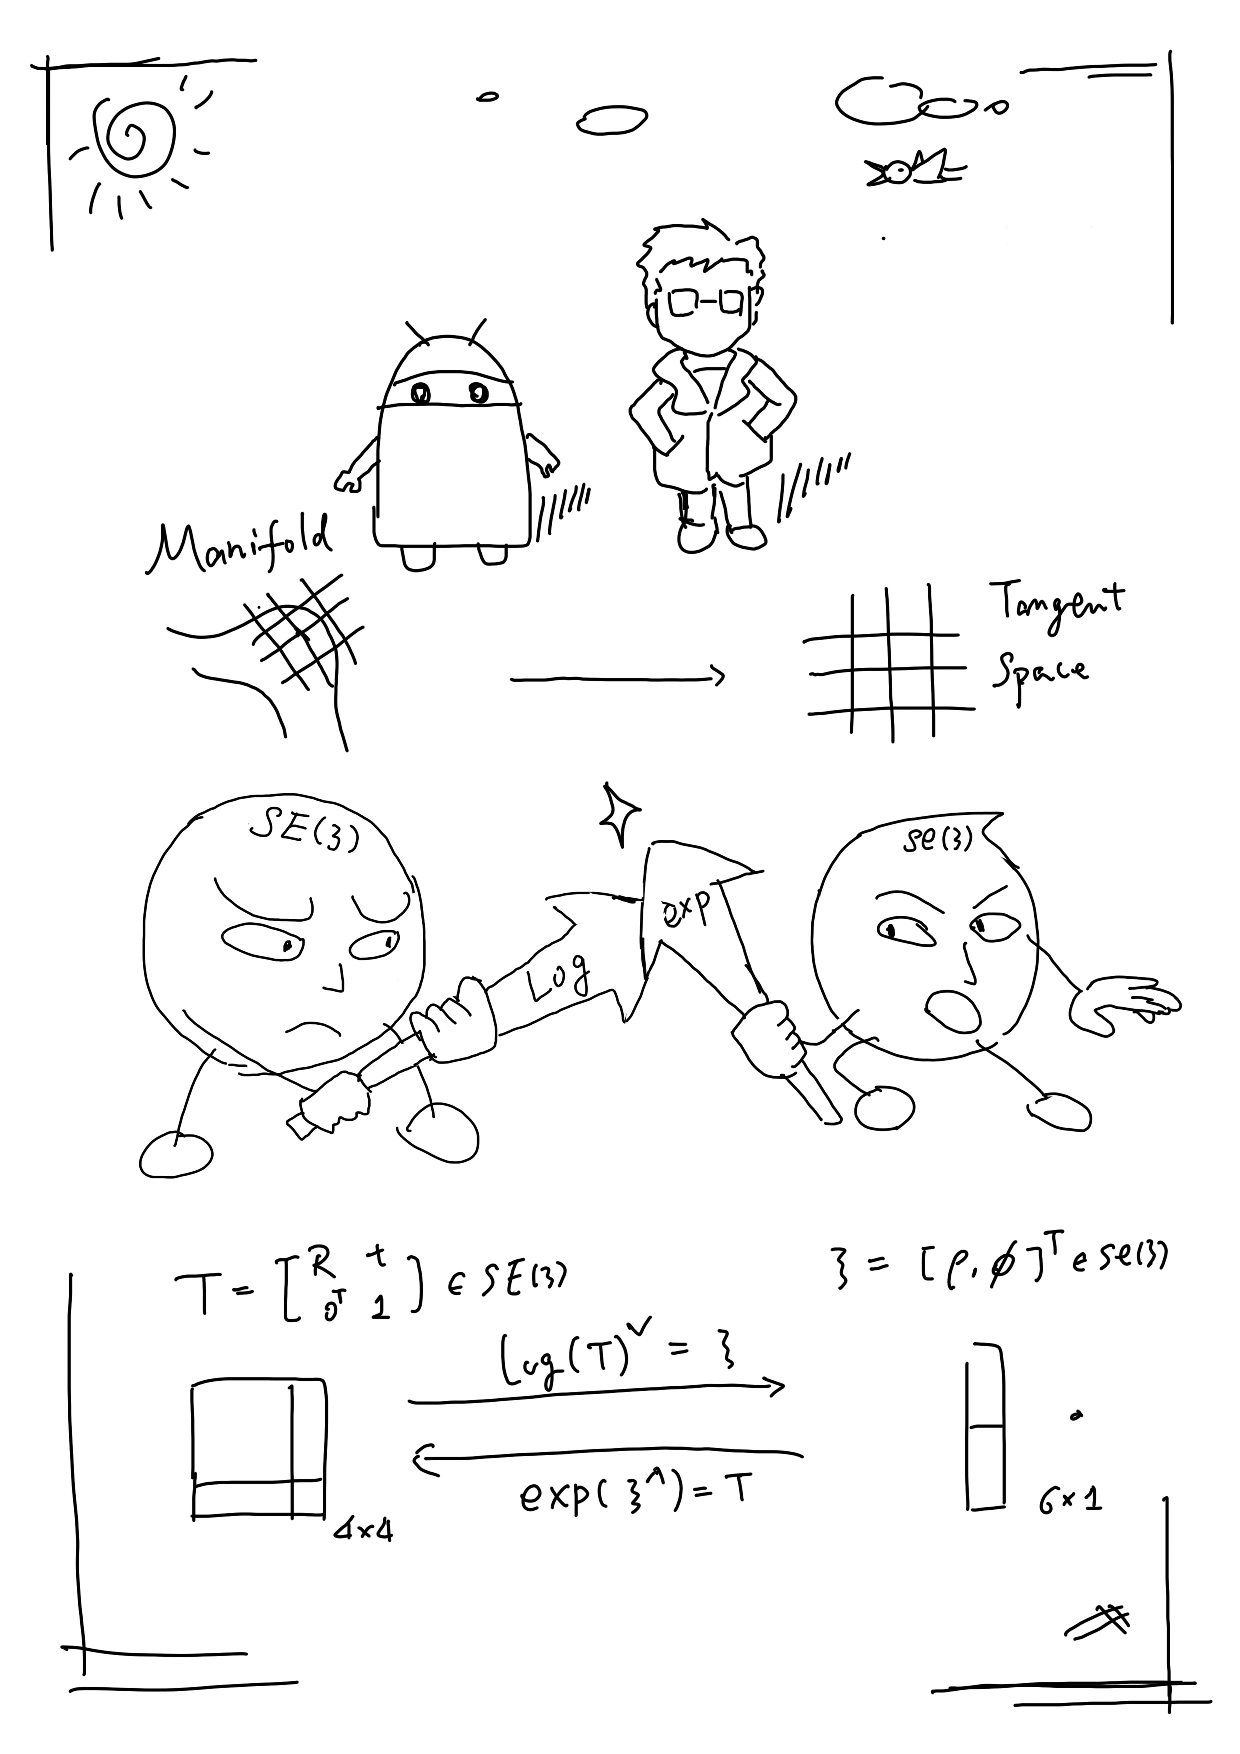
\includepdf{resources/other/ch4.pdf}
\newpage
\section{Basics of Lie Group and Lie Algebra}
In the last lecture, we introduced the definition of the rotation matrix and the transformation matrix. At the time, we said that the three-dimensional rotation matrix constitutes the \textit{special orthogonal group} $\mathrm{SO}(3)$, and the transformation matrix constitutes the \textit{special Euclidean group} $\mathrm{SE}(3) $. They are written like this:
\begin{equation}
\mathrm{SO}(3) = \{ \mathbf{R} \in \mathbb{R}^{3 \times 3} | \mathbf{RR}^T = \mathbf{I}, \det(\mathbf{R})=1 \}.
\end{equation}
\begin{equation}
\mathrm{SE}(3) = \left\{ \mathbf{T} = \left[ {\begin{array}{*{20}{c}}
    \mathbf{R} & \mathbf{t} \\
    {{\mathbf{0}^T}} & 1
    \end{array}} \right]
\in \mathbb{R}^{4 \times 4} | \mathbf{R} \in \mathrm{SO}(3), \mathbf{t} \in \mathbb{R}^3\right\}.
\end{equation}

However, at that time, we did not explain the meaning of the group in detail. Readers should note that both the rotation matrix and the transformation matrix are not closed to addition. In other words, for any two rotation matrices $\mathbf{R}_1, \mathbf{R}_2$, according to the definition, their addition is no longer a rotation matrix:
\begin{equation}
\mathbf{R}_1 + \mathbf{R}_2 \notin \mathrm{SO}(3), \quad \mathbf{T}_1 + \mathbf{T}_2 \notin \mathrm{SE}(3).
\end{equation}
You can also say that the two matrices do not have a well-defined addition operator, or the matrix addition is not closed in these two sets. The multiplication is the only one closed operation in these sets:
\begin{equation}
\mathbf{R}_1 \mathbf{R}_2 \in \mathrm{SO}(3), \quad \mathbf{T}_1 \mathbf{T}_2 \in \mathrm{SE}(3).
\end{equation}
We know that matrix multiplication corresponds to the composition of two rotations or transformations. For a set that only has one ``well-defined'' operation, we call it a \textit{group}.

\subsection{Group}
For the following contents, we need to talk a little bit about abstract algebra. I think this is a necessary condition for discussing Lie Group and Lie Algebra, but in fact, except for the students of mathematics and physics, most of the students will not have this knowledge in undergraduate classes. So let's look at some basic concepts first.

A group is an algebraic structure of one set plus one operator. We denote the set as $A$ and the operation as $\cdot$, then the group can be denoted as $G=(A,\cdot)$. We say $G$ is a \textit{group} if the operation satisfies the following conditions:

\begin{enumerate}
    \item { \textbf{Closure}}: $ \  \forall a_1, a_2 \in A, \  a_1 \cdot a_2 \in A$.
    \item { \textbf{Combination}}: $ \  \forall a_1, a_2, a_3 \in A, \  (a_1 \cdot a_2) \cdot a_3 = a_1 \cdot ( a_2 \cdot a_3) $.
    \item { \textbf{Unit element}}: $ \  \exists a_0 \in A, \  \mathrm{s.t.} \ \forall a \in A, \  a_0 \cdot a = a \cdot a_0 = a $.
    \item { \textbf{Inverse element}}: $ \  \forall a \in A, \  \exists a^{-1} \in A, \  st \  a \cdot a^{-1} = a_0 $.
\end{enumerate}

It is easy to verify that the rotation matrix set with the normal matrix multiplication form a group, the same for the transformation matrix with matrix multiplication. They can be called rotation matrix and transformation matrix groups. Other common groups include the addition of integers $(\mathbb{Z}, +)$, the rational numbers with multiplication after removing 0 $(\mathbb{Q}\backslash 0, \cdot )$, etc. Common groups in the matrix are:

\begin{itemize}
    \item {General Linear group $\mathrm{GL}(n)$}. The invertible matrix of $n \times n$ with matrix multiplication.
    \item {Special Orthogonal Group $\mathrm{SO}(n)$}. Or the rotation matrix group, where $\mathrm{SO}(2)$ and $\mathrm{SO}(3) $ is the most common.
    \item {Special Euclidean group $\mathrm{SE}(n)$}. Or the $n$ dimensional transformation described earlier, such as $\mathrm{SE}(2)$ and $\mathrm{SE}(3)$.
\end{itemize}

The group structure guarantees that the group's operations have very good properties. The group theory is the theory that studies the various structures and properties of the groups. Readers interested in group theory can refer to any of the modern algebra books. \textit{Lie Group} refers to a group with continuous (smooth) properties. Discrete groups like the integer group $\mathbb{Z}$ have no continuous properties, so they are not Lie groups. And obviously, $\mathrm{SO}(n)$ and $\mathrm{SE}(n)$ are continuous in real space because we can intuitively imagine that a rigid body moving continuously in the space, so they are all Lie Groups. Since $\mathrm{SO}(3)$ and $\mathrm{SE}(3)$ are especially important for camera pose estimation, we mainly discuss these two Lie groups. However, strictly discussing the concepts of ``continuous'' and ``smooth'' requires knowledge of analysis and topology. We don't want to write this book into a mathematics book, so only some important conclusions directly related to SLAM are introduced. If the reader is interested in the theoretical nature of Lie Groups, please refer to books like~\cite{Varadarajan2013}.

We usually have two ways to introduce the Lie Groups or Lie Algebras. The first is to directly introduce Lie group and Lie algebra and then present to the reader that each Lie group corresponds to a Lie algebra. But, in this case, the reader may think that Lie algebra seems to be a symbol that jumps out with no reason and does not know its physical meaning. So, I will take a little time to draw the Lie algebra from the rotation matrix, similar to the way of~\cite{Ma2012} and~\cite{Sola2012}. Let's start with the simpler $\mathrm{SO}(3)$, leading to the Lie algebra $\mathfrak{so}(3)$ above $\mathrm{SO}(3)$.

\subsection{Introduction of the Lie Algebra}
Consider an arbitrary rotation matrix $\mathbf{R}$, we know that it satisfies:
\begin{equation}
\mathbf{R} \mathbf{R}^T=\mathbf{I}.
\end{equation}
Now, we say that $\mathbf{R}$ is the rotation of a camera that changes continuously over time, which is a function of time: $\mathbf{R}(t)$. Since it is still a rotation matrix, we have
\[
\mathbf{R}(t) \mathbf{R}(t) ^T = \mathbf{I}.
\]
Deriving time on both sides of the equation yields (we use $\dot{\mathbf{R}}$ to represent the derivative of $\mathbf{R}$ on time $t$, just like many other control books):
\[
\dot{\mathbf{R}} (t) \mathbf{R} {(t)^T} + \mathbf{R} (t) \dot{\mathbf{R}} {(t) ^T} = 0.
\]
Move the second term to right and commute the matrices by using the transposed relation:
\begin{equation}
\dot{\mathbf{R}} (t) \mathbf{R} {(t)^T} = - \left( \dot{\mathbf{R}} (t) \mathbf{R} {(t)^T} \right)^T .
\end{equation}

It can be seen that $\dot{\mathbf{R}} (t) \mathbf{R} {(t)^T}$ is a \textit{skew-symmetric} matrix. Recall that we introduced the $^\wedge$ symbol in the cross product formula~\eqref{eq:cross}, which turns a vector into a skew-symmetric matrix. Similarly, for any skew-symmetric matrix, we can also find a unique vector corresponding to it. Let this operation be represented by the symbol $^{\vee}$:
\begin{equation}
{\mathbf{a}^ \wedge } = \mathbf{A} = \left[ {\begin{array}{*{20}{c}}
    0&{ - {a_3}}&{{a_2}}\\
    {{a_3}}&0&{ - {a_1}}\\
    { - {a_2}}&{{a_1}}&0
    \end{array}} \right], \quad
{ \mathbf{A}^ \vee } = \mathbf{a}.
\end{equation}

So, since $\dot{\mathbf{R}} (t) \mathbf{R} {(t)^T}$ is a skew-symmetric matrix, we can find a three-dimensional vector $\boldsymbol{\phi} (t) \in \mathbb{R}^3$ corresponds to it:
\[
\dot{\mathbf{R}} (t) \mathbf{R}(t)^T = \boldsymbol{\phi} (t) ^ {\wedge}.
\]

Right multiply with $\mathbf{R}(t)$ on both sides. Since $\mathbf{R}$ is an orthogonal matrix, we have:
\begin{equation}
\label{eq:dR}
\dot{\mathbf{R}} (t) = \boldsymbol{\phi} (t)^{\wedge} \mathbf{R}(t) =
\left[ {\begin{array}{*{20}{c}}
    0&{ - {\phi _3}}&{{\phi _2}}\\
    {{\phi _3}}&0&{ - {\phi _1}}\\
    { - {\phi _2}}&{{\phi _1}}&0
    \end{array}} \right] \mathbf{R} (t).
\end{equation}

It can be seen that we can take the time derivative of a ration matrix just by multiplying a $\boldsymbol{\phi}^\wedge (t)$ matrix on the left. Consider at time $t_0=0$ that the rotation matrix is $\mathbf{R}(0) = \mathbf{I}$. According to the derivative definition, we use the first-order Taylor expansion around $t=t_0$ to write $\mathbf{R}(t)$ as: 
\begin{equation}
\begin{aligned}
\mathbf{R} \left( t \right) & \approx \mathbf{R} \left( t_0 \right) + \dot {\mathbf{R}} \left( {{t_0}} \right)\left ( {t - {t_0}} \right)\\
&= \mathbf{I} + \boldsymbol{\phi} {\left( {{t_0}} \right)^ \wedge } \left( t \right).
\end{aligned}
\end{equation}

We see that $\boldsymbol{\phi}$ reflects the derivative of $\mathbf{R}$, so it is called the \textit{tangent space} near the origin of $\mathrm{SO}(3)$. 

%Also, if time $t$ is close to $t_0$, we assume $\boldsymbol{\phi}(t)$ to close to be a constant $\boldsymbol{\phi}(t_0) = \boldsymbol{\phi}_0$. Then according to the formula~\eqref{eq:dR}, we have:
%\[
%\dot{\mathbf{R}} (t) = \boldsymbol{\phi} (t_0) ^ {\wedge} \mathbf{R}(t) \approx \boldsymbol{\phi}_0^ {\wedge} \mathbf {R}(t).
%\]

The above formula is a differential equation for $\mathbf{R}$, and with the initial value $\mathbf{R}(0) = \mathbf{I}$, we have solution like:
\begin{equation}
\label{eq:so3ode}
\mathbf{R}(t) = \exp \left( \boldsymbol{\phi}_0^\wedge t \right).
\end{equation}
where we note $\boldsymbol{\phi}(t_0) = \boldsymbol{\phi}_0$.

The reader can verify that the above equation holds for both the differential equation and the initial value. This means that around $t = 0$, the rotation matrix can be calculated from $\exp \left( \boldsymbol{\phi}_0^\wedge t \right)$\footnote{At this point we have not explained what this $\exp$ means and how it works. We will talk about its definition and calculation process right after this section. }. We see that the rotation matrix $\mathbf{R}$ is associated with another skew-symmetric matrix $\boldsymbol{\phi}_0^\wedge t$ through an exponential relationship. But what is the exponential of a matrix? Here we have two questions that need to be clarified:

\begin{enumerate}
    \item Given $\mathbf{R}$ at a certain moment, we can find a $\boldsymbol{\phi}$ that describes the local derivative relationship of $\mathbf{R}$. How are they correlated with each other? We will say that $\boldsymbol{\phi}$ corresponds to the Lie algebra $\mathfrak{so}(3)$ on $\mathrm{SO}(3)$;
    \item Second, when a vector $\boldsymbol{\phi}$ is given, how is $\exp (\boldsymbol{\phi} ^\wedge )$ calculated? Conversely, given $\mathbf{R}$, is there an opposite operation to calculate $\boldsymbol{\phi}$? In fact, this is the exponential/logarithmic mapping between Lie group and Lie algebra.
\end{enumerate}

Let's solve these two problems below.

\subsection{The Definition of Lie Algebra}
Now let's give the strict definition of Lie Algebra. Each Lie group has a Lie algebra corresponding to it. Lie algebra describes the local structure of the Lie group around its origin point, or in other words, is the tangent space. The general definition of Lie algebra is listed as follows:

A Lie algebra consists of a set $\mathbb{V}$, a scalar field $\mathbb{F}$, and a binary operation $[,]$. If they satisfy the following properties, then $(\mathbb{V}, \mathbb{F}, [,])$ is a Lie algebra, denoted as $\mathfrak{g}$.

\begin{enumerate}
    \item \textbf{Closure}: $\forall \mathbf{X}, \mathbf{Y} \in \mathbb{V}; [\mathbf{X}, \mathbf{Y}] \in \mathbb{V}$.
    \item \textbf{Bilinear composition}: $\forall \mathbf{X},\mathbf{Y},\mathbf{Z} \in \mathbb{V}; a,b \in \mathbb{F }$, we have:
    \[
    [a\mathbf{X}+b\mathbf{Y}, \mathbf{Z}] = a[\mathbf{X}, \mathbf{Z}] + b [ \mathbf{Y}, \mathbf{Z} ], \quad [\mathbf{Z}, a \mathbf{X}+b\mathbf{Y}] = a [\mathbf{Z}, \mathbf{X} ]+ b [\mathbf{Z},\mathbf{Y}] .
    \]
    \item \textbf{Reflexive} \footnote{ Reflexive means that an element operates with itself results in zero. }: $\forall \mathbf{X} \in \mathbb{V}; [\mathbf{X},\mathbf{X}] = \mathbf{0}$.
    \item \textbf{Jacobi identity}: $\forall \mathbf{X},\mathbf{Y},\mathbf{Z} \in \mathbb{V}; [\mathbf{X}, [ \mathbf{Y},\mathbf{Z}] ] + [\mathbf{Z}, [\mathbf{X},\mathbf{Y}] ] + [\mathbf{Y}, [\mathbf{Z}, \mathbf{X}]] =\mathbf{0}$.
\end{enumerate}
The binary operations $[,]$ are called \textit{Lie brackets}. At first glance, we require a lot of properties about the Lie bracket.  Compared to the simpler binary operations in the group, the Lie bracket expresses the difference between the two elements. It does not require a combination law but requires the element and itself to be zero after the brackets. For example, the cross product $\times$ defined on the 3D vector $\mathbb{R}^3$ is a kind of Lie bracket, so $\mathfrak{g} = (\mathbb{R}^3, \mathbb{R}, \times)$ constitutes a Lie algebra. Readers can try to substitute the cross product into the four properties to verify the above conclusion.

\subsection{Lie Algebra $\mathfrak{so}(3)$}
The previously mentioned $\boldsymbol{\phi}$ is actually a kind of Lie algebra. The Lie algebra corresponding to $\mathrm{SO}(3)$ is a vector defined on $\mathbb{R}^3$, which we will denote as $\boldsymbol{\phi}$. According to the previous derivation, each $\boldsymbol{\phi}$ can generate a skew-symmetric matrix:
\begin{equation}
\label{eq:phi}
\boldsymbol{\varPhi} = \boldsymbol{\phi}^{\wedge} = \left[ {\begin{array}{*{20}{c}}
    0&{ - {\phi _3}}&{{\phi _2}}\\
    {{\phi _3}}&0&{ - {\phi _1}}\\
    { - {\phi _2}}&{{\phi _1}}&0
    \end{array}} \right] \in \mathbb{R}^{3 \times 3}.
\end{equation}

Under this definition, the two vectors $\boldsymbol{\phi}_1, \boldsymbol{\phi}_2$'s Lie bracket is:
\begin{equation}
[\boldsymbol{\phi}_1, \boldsymbol{\phi}_2] = \left( \mathbf{ \varPhi }_1 \mathbf{ \varPhi }_2 - \mathbf{ \varPhi }_2 \mathbf{ \varPhi }_1 \right)^\vee.
\end{equation}

Readers can verify that the Lie bracket under this definition satisfy the above properties. Since the vector $\boldsymbol{\phi}$ is one-to-one with the skew-symmetric matrix, we say the elements of $\mathfrak{so}(3)$ are three-dimensional vectors or three-dimensional skew-symmetric matrices, without any ambiguity:
\begin{equation}
\mathfrak{so}(3) = \left\{ \boldsymbol{\phi} \in \mathbb{R}^3 \ \text{or}\  \boldsymbol{\varPhi} = \boldsymbol{\phi^\wedge} \in \mathbb{ R}^{3 \times 3} \right\}.
\end{equation}

Some books also use the symbol $\widehat{\boldsymbol{\phi}}$ to represent $\boldsymbol{\phi}^\wedge$, but the meaning is the same. At this point, we have made it clear about the contents of $\mathfrak{so}(3)$. They are just a set of 3D vectors that can express the derivative of the rotation matrix. Its relationship to $\mathrm{SO}(3)$ is given by the exponential map:
\begin{equation}
\mathbf{R} = \exp ( \boldsymbol{\phi}^\wedge ).
\end{equation}
The exponential map will be introduced later. Since we have introduced $\mathfrak{so}(3)$, we will first look at the corresponding Lie algebra on $\mathrm{SE}(3)$.

\subsection{Lie Algebra $\mathfrak{se}(3)$}
For $\mathrm{SE}(3)$, it also has a corresponding Lie algebra $\mathfrak{se}(3)$. To save space, we won't start by taking time derivatives. Similar to $\mathfrak{so}(3)$, $\mathfrak{se}(3)$ is located in the $\mathbb{R}^6$ space:
\begin{equation}
\mathfrak{se}(3) = \left\{ { \boldsymbol{\xi} = \left[ \begin{array}{l}
    \boldsymbol{\rho} \\
    \boldsymbol{\phi}
    \end{array} \right]
    \in { \mathbb{R}^6} ,
    \boldsymbol{\rho} \in { \mathbb{R}^3}, \boldsymbol{\phi} \in \mathfrak{so} \left( 3 \right),{ \boldsymbol{\xi} ^ \wedge } = \left[ {\begin{array}{*{20}{c}}
        {{ \boldsymbol{\phi} ^ \wedge }}& \boldsymbol{\rho} \\
        {{\mathbf{0}^T}}&0
        \end{array}} \right] \in { \mathbb{R}^{4 \times 4}}} \right\}.
\end{equation}
We write each $\mathfrak{se}(3)$ element as $\boldsymbol{\xi}$, which is a six-dimensional vector. The first three dimensions are ``translation part'' (but keep in mind that the meaning is \textit{different} from the translation in the matrix), which is denoted as $\boldsymbol{\rho}$; the second part is a rotation part $\boldsymbol{\phi}$, which is essentially a $\mathfrak{so}(3)$ element \footnote{Please note that in some books the authors may put the rotation in the front and the translation in the back, which has no significant difference.}. At the same time, we extended the meaning of the $^\wedge$ symbol. In $\mathfrak{se}(3)$, a six-dimensional vector is converted to a four-dimensional matrix also using the $^\wedge$ symbol, but no longer a skew-symmetric one:
\begin{equation}
{ \boldsymbol{\xi} ^ \wedge } = \left[ {\begin{array}{*{20}{c}}
    {{ \boldsymbol{\phi} ^ \wedge }}& \boldsymbol{\rho} \\
    {{\mathbf{0}^T}}&0
    \end{array}} \right] \in { \mathbb{R}^{4 \times 4}}.
\end{equation}

We still use the $^\wedge$ and $^\vee$ symbols to refer to the relationship from ``vector to matrix'' and ``matrix to vector'' to maintain the consistency with $\mathfrak{so}(3)$. They are still one-to-one correspondence. The readers can simply take $\mathfrak{se}(3)$ as a ``vector consisting of a translation plus a $\mathfrak{so}(3)$ element'' (although $\boldsymbol{\rho} $ is not the direct translation). 

Finally, the Lie algebra $\mathfrak{se}(3)$ also has a Lie bracket similar to $\mathfrak{so}(3)$:
\begin{equation}
[ \boldsymbol{\xi}_1, \boldsymbol{\xi}_2 ] = \left( \boldsymbol{\xi}_1^\wedge \boldsymbol{\xi}_2^\wedge -\boldsymbol{\xi}_2^ \wedge \boldsymbol{\xi}_1^\wedge \right) ^\vee.
\end{equation}

The reader can verify that it satisfies the definition of Lie algebra (we'll leave it as an exercise). So far we have seen two important Lie algebras $\mathfrak{so}(3)$ and $\mathfrak{se}(3)$.

\section{Exponential and Logarithmic Mapping}
\subsection{Exponential Map of $\mathrm{SO}(3)$}

Now consider the second question: How to calculate $\exp ( \boldsymbol{\phi}^{\wedge} )$? In other words, it is an exponential map of a matrix. Again, we will first discuss the exponential mapping of $\mathfrak{so}(3)$ and then the case of $\mathfrak{se}(3)$.

The exponential of an arbitrary matrix can be written as a Taylor expansion if it has converged, whose result is still a matrix:
\begin{equation}
\exp(\mathbf{A}) = \sum\limits_{n = 0}^\infty {\frac{1}{{n!}}{ \mathbf{A}^n}}.
\end{equation}

Similarly, for any element in $\boldsymbol{\phi} \in \mathfrak{so}(3)$, we can also define its exponential map in this way:
\begin{equation}
\exp(\boldsymbol{\phi}^\wedge) = \sum\limits_{n = 0}^\infty {\frac{1}{{n!}}{ (\boldsymbol{\phi}^{\wedge })^n}}.
\end{equation}
But this definition cannot be calculated directly because we don't want to calculate the infinite power of a matrix. Below we derive a convenient way to calculate the exponential mapping. Since $\boldsymbol{\phi}$ is a three-dimensional vector, we can define its length and direction,  denoted as $\theta$ and $\mathbf{n}$, respectively. So we have $\boldsymbol{\phi} = \theta \mathbf{n}$, where $\mathbf{n}$ is a unit-length direction vector, i.e., $\| \mathbf{n} \| =1$. First, for such a unit-length vector $\mathbf{n}$, there are two properties:
\begin{equation}
 \mathbf{n}^{\wedge} \mathbf{n}^{\wedge} = \left[ {\begin{array}{*{20}{c}}
{ - n_2^2 - n_3^2}&{{n_1}{n_2}}&{{n_1}{n_3}}\\
{{n_1}{n_2}}&{ - n_1^2 - n_3^2}&{{n_2}{n_3}}\\
{{n_1}{n_3}}&{{n_2}{n_3}}&{ - n_1^2 - n_2^2}
\end{array}} \right] = \mathbf{n} \mathbf{n}^T - \mathbf{I},
\end{equation}
as well as
\begin{equation}
\mathbf{n}^{\wedge} \mathbf{n}^{\wedge} \mathbf{n}^{\wedge} = \mathbf{n}^\wedge (\mathbf{n}\mathbf{n} ^T-\mathbf{I}) = \underbrace{\mathbf{n}^\wedge \mathbf{n}}_{\text{zero}} \mathbf{n}^T - \mathbf{n}^{\wedge} = - \mathbf{n}^{\wedge}.
\end{equation}
These two formulas provide a way to handle the high-order $\mathbf{n}^\wedge$ items. Now we can write the exponential map as:
\begin{align*}
\exp \left( {{\boldsymbol{\phi} ^ \wedge }} \right) &= \exp \left( {\theta {\mathbf{n}^ \wedge }} \right) = \sum\limits_ {n = 0}^\infty {\frac{1}{{n!}}{{\left( {\theta {\mathbf{n}^ \wedge }} \right)}^n}} \\
&= \mathbf{I} + \theta {\mathbf{n}^ \wedge } + \frac{1}{{2!}}{\theta ^2}{\mathbf{n}^ \wedge }{\mathbf{n}^ \wedge } + \frac{1}{{3!}}{\theta ^3}{\mathbf{n}^ \wedge }{\mathbf{n}^ \wedge }{\mathbf{n}^ \wedge } + \frac{1}{{4!}}{\theta ^4}{\left( {{\mathbf{n}^ \wedge }} \right)^4} + ... \\
&= \mathbf{n} {\mathbf{n}^T} - {\mathbf{n}^ \wedge }{\mathbf{n}^ \wedge } + \theta {\mathbf{n} ^ \wedge } + \frac{1}{{2!}}\theta^2 {\mathbf{n}^ \wedge }{\mathbf{n}^ \wedge } - \frac{1}{{3! }}{\theta ^3}{\mathbf{n}^ \wedge } - \frac{1}{{4!}}{\theta ^4}{\left( {{\mathbf{n}^ \wedge }} \right)^2} + ...\\
&= \mathbf{n}{\mathbf{n}^T} + \underbrace{\left( {\theta - \frac{1}{{3!}}{\theta ^3} + \frac{1}{{5!}}{\theta ^5} - ...} \right)}_{\sin \theta} {\mathbf{n}^ \wedge } - \underbrace{\left( { 1 - \frac{1}{{2!}}{\theta ^2} + \frac{1}{{4!}}{\theta ^4} - ...} \right)}_{\cos \theta}{\mathbf{n}^ \wedge }{\mathbf{n}^ \wedge }\\
&= {\mathbf{n}^ \wedge }{\mathbf{n}^ \wedge } + \mathbf{I} + \sin \theta {\mathbf{n}^ \wedge } - \cos \theta {\mathbf{n}^ \wedge }{\mathbf{n}^ \wedge }\\
&= (1 - \cos \theta ){\mathbf{n}^ \wedge }{\mathbf{n}^ \wedge } + \mathbf{I} + \sin \theta {\mathbf{n}^ \wedge }\\
&= \cos \theta \mathbf{I} + (1 - \cos \theta )\mathbf{n}{\mathbf{n}^T} + \sin \theta {\mathbf{n}^ \wedge }.
\end{align*}

Finally, we get a very familiar equation:
\begin{equation}
\exp( \theta \mathbf{n}^\wedge ) = \cos \theta \mathbf{I} + (1 - \cos \theta )\mathbf{n}{\mathbf{n}^T } + \sin \theta {\mathbf{n}^ \wedge }.
\end{equation}

Recall the previous lesson. This equation is exactly the same as Rodrigues' formula, i.e., equation \eqref{eq:rogridues}. This shows that $\mathfrak{so}(3)$ is actually the \textit{rotation vector}, and the exponential map is just Rodrigues' formula. Through them, we map any vector in $\mathfrak{so}(3)$ to a rotation matrix in $\mathrm{SO}(3)$. Conversely, if we define a logarithmic map, we can also map the elements in $\mathrm{SO}(3)$ to $\mathfrak{so}(3)$:
\begin{equation}
\boldsymbol{\phi} = \ln {\left( \mathbf{R} \right)^ \vee } = {\left( {\sum\limits_{n = 0}^\infty {\frac{{{{ \left( { - 1} \right)}^n}}}{{n + 1}}{{\left( { \mathbf{R} - \mathbf{I}} \right)}^{n + 1 }}} } \right)^ \vee }.
\end{equation}
Just like the exponential mapping, we have to use the Taylor series to expand the logarithmic mapping. In Lecture 3, we have already introduced how to calculate the corresponding Lie algebra according to the rotation matrix, that is, using the formula \eqref{eq:R2theta}, and use the properties of the trace to solve the rotation angle and the rotation axis separately, which is more convenient.

Now, we've introduced the calculation method of exponential mapping. Readers may ask, what is the property of the exponential mapping? Can I find a unique $\boldsymbol{\phi}$ for any $\mathbf{R}$? Unfortunately, the exponential map is just a surjective map, not injective. This means that for each element in $\mathrm{SO}(3)$ we can find a $\mathfrak{so}(3)$ element corresponding to it; however, there may be multiple $\mathfrak{so}(3)$ elements corresponding to the same $\mathrm{SO}(3)$ element. At least for the rotation angle $\theta$, we know that rotating multiple $360^\circ$ will give the same rotation - it has periodicity. However, if we fix the rotation angle between $\pm \pi$, then the Lie group and the Lie algebra elements are one-to-one correspondence.

The conclusion of $\mathrm{SO}(3)$ and $\mathfrak{so}(3)$ seems to be in our expectation. It is very similar to the rotation vector we talked about earlier, and the exponential mapping is the Rodrigues formula. The derivative of the rotation matrix can be specified by the rotation vector, which guides how to perform calculus operations in the rotation matrix.

\subsection{Exponential Map of $\mathrm{SE}(3)$}

The exponential map on $\mathfrak{se}(3)$ is described below. To save space, we no longer deduct the exponential mapping in detail like $\mathfrak{so}(3)$. The exponential mapping on $\mathfrak{se}(3)$ is as follows:
\begin{align}
\exp \left( {{ \boldsymbol{\xi} ^ \wedge }} \right) &= \left[ {\begin{array}{*{20}{c}}
    {\sum\limits_{n = 0}^\infty {\frac{1}{{n!}}{{\left( {{\boldsymbol{\phi} ^ \wedge }} \right)}^n} } }&{\sum\limits_{n = 0}^\infty {\frac{1}{{\left( {n + 1} \right)!}}{{\left( {{\boldsymbol{\phi } ^ \wedge }} \right)}^n} \boldsymbol{\rho} } }\\
    {{\mathbf{0}^T}}&1
    \end{array}} \right] \\
&\buildrel \Delta \over = \left[ {\begin{array}{*{20}{c}}
    \mathbf{R} &{\mathbf{J\rho} } \\
    {{\mathbf{0}^T}}&1
    \end{array}} \right] = \mathbf{T}.
\end{align}

With a little patience, you can derive the Taylor expansion from the practice of $\mathfrak{so}(3)$. Let $\boldsymbol{\phi}=\theta \mathbf{a}$, where $\mathbf{a}$ is the unit vector, then:
\begin{equation}
\begin{aligned}
\sum\limits_{n = 0}^\infty {\frac{1}{{\left( {n + 1} \right)!}}{{\left( {{\boldsymbol{\phi} ^ \wedge }} \right)}^n}} &= \mathbf{I} + \frac{1}{{2!}}\theta {\mathbf{a}^ \wedge } + \frac{1}{{3 !}}{\theta ^2}{\left( {{\mathbf{a}^ \wedge }} \right)^2} + \frac{1}{{4!}}{\theta ^3}{ \left( {{\mathbf{a}^ \wedge }} \right)^3} + \frac{1}{{5!}}{\theta ^4}{\left( {{\mathbf{a} ^ \wedge }} \right)^4} \cdots \\
&= \frac{1}{\theta }\left( {\frac{1}{{2!}}{\theta ^2} - \frac{1}{{4!}}{\theta ^4} + \cdots } \right)\left( {{\mathbf{a}^ \wedge }} \right) + \frac{1}{\theta }\left( {\frac{1}{{3!}} {\theta ^3} - \frac{1}{5}{\theta ^5} + \cdots } \right){\left( {{\mathbf{a}^ \wedge }} \right)^2} + \mathbf{I}\\
&= \frac{1}{\theta }\left( {1 - \cos \theta } \right)\left( {{\mathbf{a}^ \wedge }} \right) + \frac{{\theta - \sin \theta }}{\theta }\left( {\mathbf{a}{\mathbf{a}^T} - \mathbf{I}} \right) + \mathbf{I}\\
&= \frac{{\sin \theta }}{\theta }\mathbf{I} + \left( {1 - \frac{{\sin \theta }}{\theta }} \right)\mathbf{a }{\mathbf{a}^T} + \frac{{1 - \cos \theta }}{\theta }{\mathbf{a}^ \wedge } \buildrel \Delta \over = \mathbf{J}.
\end{aligned}
\end{equation}

From the results, we can see the $\mathbf{R}$ in the upper left corner of the exponential map of $\boldsymbol{\xi}$ is just the well-known $\mathrm{SO}(3)$, which means the rotation part of $\boldsymbol{\xi}$ is just the rotation part in $\mathfrak{so}(3)$. The $\mathbf{J}$ in the upper right corner is given by the above derivation:
\begin{equation}
\label{eq:lieAlgebraJacobian}
\mathbf{J} = \frac{{\sin \theta }}{\theta } \mathbf{I} + \left( {1 - \frac{{\sin \theta }}{\theta }} \right) \mathbf{a} { \mathbf{a}^T} + \frac{{1 - \cos \theta }}{\theta }{ \mathbf{a}^ \wedge }.
\end{equation}

This formula is somewhat similar to the Rodrigues formula but not exactly the same. We see that after passing the exponential map, the translation part is multiplied by a linear jacobian matrix $\mathbf{J}$. Please pay attention to the $\mathbf{J}$ here, as it will be used later.

Similarly, although we can also derive the logarithmic mapping analytically, there is a more trouble-free way to find the corresponding vector on $\mathfrak{so}(3)$ according to the transformation matrix $\mathbf{T}$: from the upper left corner $\mathbf{R}$ we can calculate the rotation vector, while $\mathbf{t}$ the upper right corner satisfies:
\begin{equation}
\mathbf{t} = \mathbf{J} \boldsymbol{\rho}.
\end{equation}

Since $\mathbf{J}$ can be obtained from $\boldsymbol{\phi}$, $\boldsymbol{\rho}$ can also be solved by this linear equation. Now, we have clarified the definition of Lie group and Lie algebra and their mutual conversion relationship, as summarized in \autoref{fig:liegroupandAlgebra}~. If the reader doesn't understand everything, please go back to a few pages to read through the derivation again.

\begin{figure}[!ht]
    \centering
    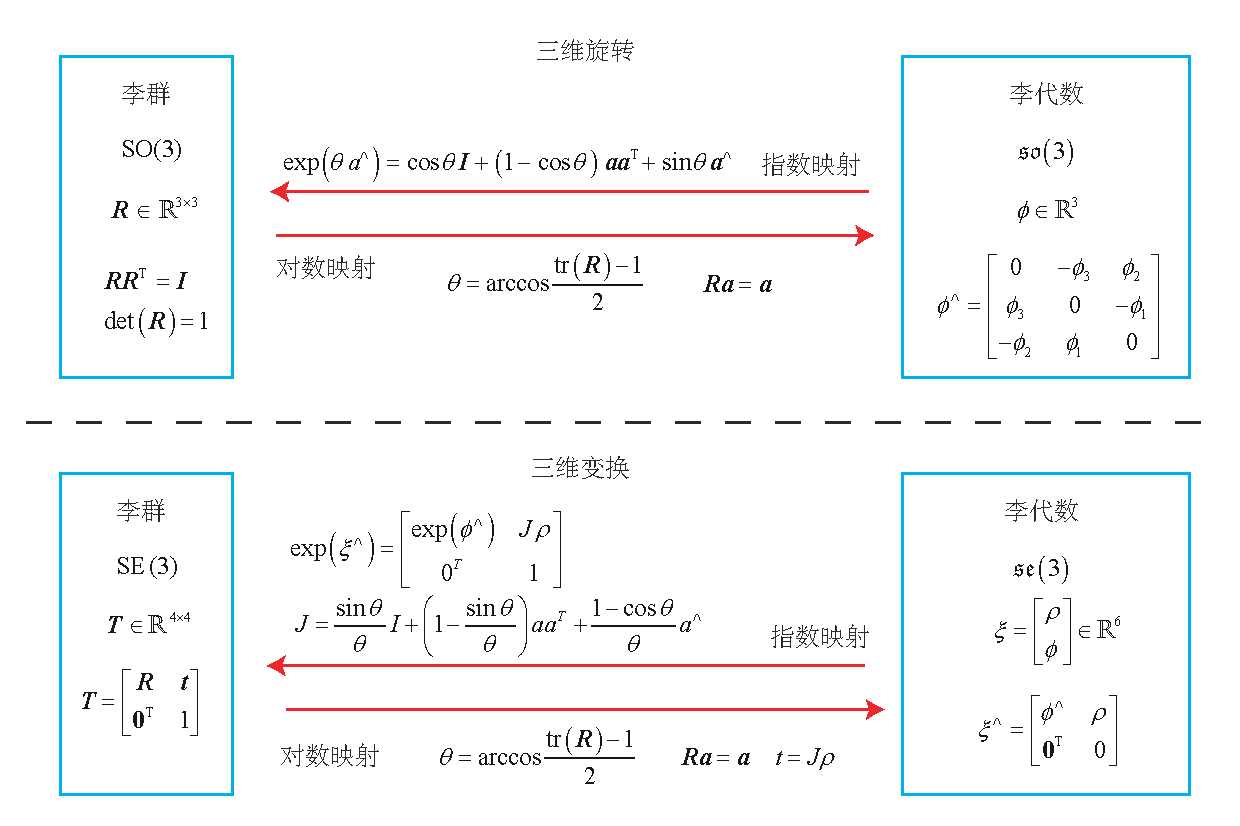
\includegraphics[width=1.0\textwidth]{lieGroup/liegroupandAlgebra.pdf}
    \caption{The correspondence between $\mathrm{SO}(3), \mathrm{SE}(3), \mathfrak{so}(3), \mathfrak{se}(3)$. }
    \label{fig:liegroupandAlgebra}
\end{figure}

\section{Lie Algebra Derivation and Perturbation Model}
\subsection{BCH Formula and its Approximation}
A major motivation for using Lie algebra is to do optimization. The derivative is a very necessary part of the optimization process (we will talk about it in detail in lecture~\ref{cpt:6}). Let's consider the problem below. Although we have already understood the relationship between Lie group and Lie algebra on $\mathrm{SO}(3)$ and $\mathrm{SE}(3)$, but what happens in $\mathfrak{so}(3)$ when two matrices are multiplied in $\mathrm{SO}(3)$? Conversely, when we add two vectors in $\mathfrak{so}(3)$, does $\mathrm{SO}(3)$ correspond to the product of the two matrices? If we write it out, it should be:
\[
\exp \left( {\boldsymbol{\phi}_1^\wedge } \right)\exp \left( {\boldsymbol{\phi}_2^\wedge}\right) = \exp \left( {{{\left( {{\boldsymbol{\phi} _1} + {\boldsymbol{\phi} _2}} \right)}^ \wedge }} \right) ?
\]

If $\boldsymbol{\phi}_1, \boldsymbol{\phi}_2$ are scalars, then this is obviously true; but here we calculate the exponential map of \textit{matrices} instead of scalars. In other words, we are studying whether the following formula holds:
\[
\ln \left( \exp \left( \mathbf{A} \right) \exp \left( \mathbf{B} \right) \right) = \mathbf{A} + \mathbf{B} \; ?
\]
for matrices. Unfortunately, this formula is not true in the matrix. The complete form of the product is given by the Baker-Campbell-Hausdorff formula (BCH formula)\footnote{ See \url{https://en.wikipedia.org/wiki/Baker-Campbell-Hausdorff\_formula}. }. Due to the complexity of its complete form, we only give the first few items of its expansion:
\begin{equation}
\ln \left( {\exp \left( \mathbf{A} \right)\exp \left( \mathbf{B} \right)} \right) = \mathbf{A} + \mathbf{B} + \frac{1}{2}\left[ {\mathbf{A}, \mathbf{B}} \right] + \frac{1}{{12}}\left[ {\mathbf{A},\left[ {\mathbf{A}, \mathbf{B}} \right]} \right] - \frac{1}{{12}}\left[ {\mathbf{B},\left[ {\mathbf{A} ,\mathbf{B}} \right]} \right] + \cdots
\end{equation}
where $[]$ is the Lie brackets. The BCH formula tells us that how to deal with the product of two matrices: they produce some extra Lie brackets compared with the scalar form. In particular, consider the case of $\mathrm{SO}(3)$ and $\ln { \left( {\exp \left( { \boldsymbol{\phi} _1^ \wedge } \right)\exp \left ( {\boldsymbol{\phi} _2^ \wedge } \right)} \right) ^ \vee }$, when $\boldsymbol{\phi_1}$ or $\boldsymbol{\phi_2}$ is small. Small items with more than quadratic can be  ignored when taking derivatives. At this time, BCH has a linear approximation\footnote{We are not going to do the detailed derivation of BCH approximation, see~\cite{Barfoot2016} if you are interested. }:
\begin{equation}
\ln { \left( {\exp \left( { \boldsymbol{\phi} _1^ \wedge } \right)\exp \left( {\boldsymbol{\phi} _2^ \wedge } \right)} \right ) ^ \vee } \approx \left\{
\begin{array}{l}
{\mathbf{J}_l}{\left( {{\boldsymbol{\phi} _2}} \right)^{ - 1}}{ \boldsymbol{\phi} _1} + {\boldsymbol{\phi} _2 } \quad \text{when} \ \boldsymbol{\phi}_1 \ \text{is a small amount},\\
{\mathbf{J}_r}{\left( {{\boldsymbol{\phi} _1}} \right)^{ - 1}}{\boldsymbol{\phi} _2} + {\boldsymbol{\phi} _1 } \quad \text{when} \  \boldsymbol{\phi}_2 \ \text{is a small amount}.
\end{array} \right.
\end{equation}

Take the first approximation as an example. This formula tells us that left multiplying a tiny rotation matrix $\mathbf{R}_1$ on a rotation matrix $\mathbf{R}_2$ (whose Lie algebra is $\boldsymbol{\phi}_1$ and $\boldsymbol{\phi}_2$, respectively), in $\mathfrak{so}(3)$ it can be approximated by adding a $\mathbf{J}_l \left( {\boldsymbol{\phi} _2} \right)^{ - 1} { \boldsymbol{\phi} _1}$ to the original Lie algebra $\boldsymbol{\phi}_2$.  Similarly, the second approximation describes the case where $\mathbf{R}_1$ is right multiplied by a small rotation. Therefore, under the BCH approximation, the Lie algebra is divided into a left-multiplying approximation and a right-multiplying approximation. We must pay attention to whether the left model or the right model is used in daily usage. This book takes the left multiplication as an example. The jacobian in our left model $\mathbf{J}_l$ is exactly the content of the form \eqref{eq:lieAlgebraJacobian}~:
\begin{equation}
{ \mathbf{J}_l} = \mathbf{J} = \frac{{\sin \theta }}{\theta } \mathbf{I} + \left( {1 - \frac{{\sin \theta } }{\theta }} \right) \mathbf{a} { \mathbf{a}^T} + \frac{{1 - \cos \theta }}{\theta }{ \mathbf{a} ^ \wedge}.
\end{equation}

Its inverse is:
\begin{equation}
\mathbf{J}_l^{ - 1} = \frac{\theta }{2}\cot \frac{\theta }{2} \mathbf{I} + \left( {1 - \frac{\theta } {2}\cot \frac{\theta }{2}} \right) \mathbf{a} {\mathbf{a}^T} - \frac{\theta }{2}{ \mathbf{ a}^ \wedge },
\end{equation}
when $\theta$ is not zero (in that case we take both $\mathbf{J}_{l}$ and its inverse as identity). To get the right jacobian we only need to take a negative sign for the argument:
\begin{equation}
\mathbf{J}_r(\boldsymbol{\phi}) =\mathbf{J}_l(-\boldsymbol{\phi}) .
\end{equation}

In this way, we've made it clear about the relationship between Lie group multiplication and Lie algebra addition.

For the convenience, we restate the meaning of the BCH approximation. Suppose we have a rotation $\mathbf{R}$, the corresponding Lie algebra is $\boldsymbol{\phi}$. We give it a small perturbation to the left, denoted as $\Delta \mathbf{R}$, and so that the corresponding Lie algebra is $\Delta \boldsymbol{\phi}$. Then, on Lie group, the result is $ \Delta \mathbf{R} \cdot \mathbf{R}$, and on the Lie algebra, according to the BCH approximation, it is $\mathbf{J}_l^{-1 } (\boldsymbol{\phi}) \Delta \boldsymbol{\phi} + \boldsymbol{\phi}$. Putting them together, we can simply write:
\begin{equation}
\exp \left( {\Delta { \boldsymbol{\phi} ^ \wedge }} \right)\exp \left( {{ \boldsymbol{\phi} ^ \wedge }} \right) = \exp \left( {{{\left( { \boldsymbol{\phi} + \mathbf{J}_l^{ - 1}\left( \boldsymbol{\phi} \right)\Delta \boldsymbol{\phi} } \right)} ^ \wedge }} \right).
\end{equation}

Conversely, if we do addition on Lie algebra by adding $\boldsymbol{\phi}$ with $\Delta \boldsymbol{\phi}$, we can approximate the multiplication on the Lie group as:
\begin{equation}
\exp \left( {{{\left( { \boldsymbol{\phi} + \Delta \boldsymbol{\phi} } \right)}^ \wedge }} \right) = \exp \left( {{{\left( {{ \mathbf{J}_l}\Delta \boldsymbol{\phi} } \right)}^ \wedge }} \right)\exp \left( {{ \boldsymbol{\phi} ^ \wedge }} \right) = \exp \left( {{\boldsymbol{\phi} ^ \wedge }} \right)\exp \left( {{{\left( {{\mathbf{J}_r}\Delta \boldsymbol{ \phi} } \right)}^ \wedge }} \right).
\end{equation}

This provides a theoretical basis for calculus on Lie algebra. Similarly, for $\mathrm{SE}(3)$, there is a similar BCH approximation:
\begin{equation}
\exp \left( {\Delta {\boldsymbol{\xi} ^ \wedge }} \right)\exp \left( {{ \boldsymbol{\xi} ^ \wedge }} \right) \approx \exp \left ( {{{\left( {{ \boldsymbol{\mathcal{J}}_l^{-1} }\Delta \boldsymbol{\xi} + \boldsymbol{\xi} } \right)}^ \wedge }} \right),
\end{equation}
\begin{equation}
\exp \left( {{ \boldsymbol{\xi} ^ \wedge }} \right) \exp \left( {\Delta {\boldsymbol{\xi} ^ \wedge }} \right) \approx \exp \left ( {{{\left( {{ \boldsymbol{\mathcal{J}}_r^{-1} }\Delta \boldsymbol{\xi} + \boldsymbol{\xi} } \right)}^ \wedge }} \right).
\end{equation}

Here the $\boldsymbol{\mathcal{J}}_l$ and $\boldsymbol{\mathcal{J}}_r$ are more complicated $6 \times 6$ matrices. Readers can find its detailed contents in~\cite{Barfoot2016}. Since we did not use these two jacobians matrices in the calculation (we will see in the next subsection), the exact form is omitted here.

\subsection{Derivative on $\mathrm{SO}(3)$}
Now let's talk about how to compute the derivation if our target function is related to a rotation or a transform, which has a powerful practical meaning since we usually have these functions to optimize in solving the SLAM problem. Assume we want to estimate a pose described by $\mathrm{SO}(3)$ or $\mathrm{SE}(3)$ elements. Our robot observes a point with the world coordinate $\mathbf{p}$ and generates an observation data $\mathbf{z}$, which can be written as:
\begin{equation}
\mathbf{z} = \mathbf{T} \mathbf{p} + \mathbf{w},
\end{equation}
where $\mathbf{w}$ is the noise (and is unknown). Because of the noise, the real observed data is not absolutely the same as the one we computed from the observation model, so we can calculate the error of predicted observation with the real one: 
\begin{equation}
\mathbf{e} = \mathbf{z} - \mathbf{T} \mathbf{p}.
\end{equation}

Suppose we have $N$ points in total, then we find a best $\mathbf{T}$ to make the error minimized: 
\begin{equation}
\mathop {\min }\limits_{\mathbf{T}} J(\mathbf{T} ) = \sum_{i=1}^{N} \left\| {\mathbf{z}_i - \mathbf{Tp}_i} \right\|^2_2.
\end{equation}

Because of the noise, the real observed data is not absolutely the same as the one we computed from the observation model, so we can calculate the error of predicted observation with the real one: 
To solve such an optimized problem (which is a least square problem), we need to calculate the derivative of $J$ by $\mathbf{T}$. We leave the least square problem to the next section. Here we just want to clarify that we normally have some functions that have rotations or transforms as their variables. We have to adjust those rotations or transforms to find a better/best estimation. But, as we mentioned before, since $\mathrm{SO}(3)$ and $\mathrm{SE}(3)$ do not have a well-defined addition (they are just groups), so the derivatives cannot be defined in their common form. If we treat the $\mathbf{R}$ or $\mathbf{T}$ as common matrices, we have to introduce the constraints into our optimization. 

However, from the perspective of Lie algebra, since it consists of vectors, it has a good addition operation. Therefore, there are two ways to solve the problem of derivation using Lie algebra:

\begin{enumerate}
    \item Assume we add a infinitesimal amount on Lie algebra, then compute the change of the object function.
    \item Assume we multiply an infinitesimal perturbation on the Lie group left multiplication or right multiplication, use Lie algebra to describe the perturbation, and then compute the derivative on this perturbation. This is called as left perturbation or right perturbation model.
\end{enumerate}

The first method corresponds to the normal derivation model of the Lie algebra, and the second corresponds to the perturbation model. Let's discuss the similarities and differences between these two approaches.

\subsection{Derivative Model}
First, consider the situation on $\mathrm{SO}(3)$. Suppose we rotate a space point $\mathbf{p}$ and get $\mathbf{R} \mathbf{p}$. To calculate the derivative of the point coordinates by the rotation, we informally write it as \footnote{Please note that the derivative cannot be defined by matrix differentiation. Here we just write it for convenience. }:
\[
\frac{{\partial \left( {\mathbf{Rp}} \right)}}{{\partial \mathbf{R}}}.
\]
Since $\mathrm{SO}(3)$ has no addition operator, it cannot be calculated by the common derivative definition. Let the Lie algebra corresponding to $\mathbf{R}$ be $\boldsymbol{\phi}$, and we will calculate instead of the common derivative:\footnote{Strictly speaking, in matrix differentiation, we can only compute the derivative of a row vector to a column vector, whose result is a matrix. However, in this book, we write the derivative of the column vector to the column vector for convenience. The reader can think that the numerator is transposed first, and after the computation, the final result is also transposed (see appendix~\ref{cpt:app-B} for details). This makes the formula look simple; otherwise, we have to add a transpose to each equation. In this sense, we can use equations like $\mathrm{d}(\mathbf{Ax})/\mathrm{d}\mathbf{x} = \mathbf{A}$. }:
\[ \frac{{\partial \left( {\exp \left( \boldsymbol{\phi} ^ \wedge \right) \mathbf{p}} \right)}}{{\partial \boldsymbol{\phi} }}. \]

%\clearpage
According to the definition of the derivative, we have:
\begin{align*}
\frac{{\partial \left( {\exp \left( {{ \boldsymbol{\phi} ^ \wedge }} \right) \mathbf{p}} \right)}}{{\partial \boldsymbol{\phi} }} &= \mathop {\lim }\limits_{\delta \boldsymbol{\phi}  \to \mathbf{0}} \frac{{\exp \left( {{{\left( {\boldsymbol{\phi}  + \delta \boldsymbol{\phi} } \right)}^ \wedge }} \right) \mathbf{p} - \exp \left( {{\boldsymbol{\phi} ^ \wedge }} \right)\mathbf{p}}}{{\delta \boldsymbol{\phi} }}\\
& = \mathop {\lim }\limits_{\delta \boldsymbol{\phi}  \to \mathbf{0}} \frac{{\exp \left( {{{\left( {{\mathbf{J}_l}\delta \boldsymbol{\phi} } \right)}^ \wedge }} \right)\exp \left( {{\boldsymbol{\phi} ^ \wedge }} \right) \mathbf{p} - \exp \left( {{\boldsymbol{\phi} ^ \wedge }} \right) \mathbf{p}}}{{\delta \boldsymbol{\phi} }}\\
&= \mathop {\lim }\limits_{\delta \boldsymbol{\phi}  \to \mathbf{0}} \frac{{\left( { \mathbf{I} + {{\left( {{ \mathbf{J}_l}\delta \boldsymbol{\phi} } \right)}^ \wedge }} \right)\exp \left( {{\boldsymbol{\phi} ^ \wedge }} \right) \mathbf{p} - \exp \left( {{\boldsymbol{\phi} ^ \wedge }} \right)\mathbf{p}}}{{\delta \boldsymbol{\phi} }}\\
&= \mathop {\lim }\limits_{\delta \boldsymbol{\phi}  \to \mathbf{0}} \frac{{{{\left( {{\mathbf{J}_l}\delta \boldsymbol{\phi} } \right)}^ \wedge }\exp \left( {{\boldsymbol{\phi} ^ \wedge }} \right)\mathbf{p}}}{{\delta \boldsymbol{\phi} }}\\
&= \mathop {\lim }\limits_{\delta \boldsymbol{\phi}  \to \mathbf{0}} \frac{{ - {{\left( {\exp \left( {{\boldsymbol{\phi} ^ \wedge }} \right)\mathbf{p}} \right)}^ \wedge }{\mathbf{J}_l}\delta \boldsymbol{\phi} }}{{\delta \boldsymbol{\phi}}} =  - {\left( {\mathbf{Rp}} \right)^ \wedge }{\mathbf{J}_l}.
\end{align*}

The second line is BCH approximation. The third line is Taylor's approximation after throwing the high-order terms (but we still write the equal sign here because the limit is taken). The fourth to the fifth line treat the skew-symmetric symbol as a cross-product so that $\mathbf{a} \times \mathbf{b} = -\mathbf{b} \times \mathbf{a}$. Thus, we compute the derivative of the rotated point relative to the addition in Lie algebra:
\begin{equation}
\frac{{\partial \left( { \mathbf{Rp}} \right)}}{{\partial \boldsymbol{\phi} }} = {\left( { - \mathbf{Rp}} \right)^ \wedge }{\mathbf{J}_l}.
\end{equation}

However, since there is still a very complicated form of $\mathbf{J}_l$, we don't want to calculate it. The perturbation model described below provides a more straightforward way to compute derivatives.

\subsection{Perturbation Model}
Another way to do this is to perturb $\mathbf{R}$ by $\Delta \mathbf{R}$ and see the change of the result relative to the disturbance. This disturbance can be multiplied on the left or on the right. The final result will be slightly different. Let's take the left perturbation as an example. Let the left perturbation $\Delta \mathbf{R}$ correspond to the Lie algebra as $\boldsymbol{\varphi}$. Then, for $\boldsymbol{\varphi}$, that is:
\begin{equation}
\frac{{\partial \left( {\mathbf{Rp}} \right)}}{{\partial \boldsymbol{\varphi} }} = \mathop {\lim }\limits_{\boldsymbol{\varphi}  \to \mathbf{0}} \frac{{\exp \left( {{\boldsymbol{\varphi} ^ \wedge }} \right)\exp \left( {{\boldsymbol{\phi} ^ \wedge }} \right)\mathbf{p} - \exp \left( {{\boldsymbol{\phi} ^ \wedge }} \right)\mathbf{p}}}{\boldsymbol{\varphi} }.
\end{equation}

The derivation of this formula is simpler than the above:
\begin{align*}
\frac{{\partial \left( {\mathbf{Rp}} \right)}}{{\partial \boldsymbol{\varphi} }} &= \mathop {\lim }\limits_{\boldsymbol{\varphi}  \to \mathbf{0}} \frac{{\exp \left( {{\boldsymbol{\varphi} ^ \wedge }} \right)\exp \left( {{\boldsymbol{\phi} ^ \wedge }} \right)\mathbf{p} - \exp \left( {{\boldsymbol{\phi} ^ \wedge }} \right)\mathbf{p}}}{ \boldsymbol{\varphi} }\\
&= \mathop {\lim }\limits_{\boldsymbol{\varphi } \to \mathbf{0}} \frac{{\left( {\mathbf{I} + {\boldsymbol{\varphi }^ \wedge }} \right)\exp \left( {{\boldsymbol{\phi} ^ \wedge }} \right)\mathbf{p} - \exp \left( {{\boldsymbol{\phi} ^ \wedge }} \right)\mathbf{p}}}{\boldsymbol{\varphi} }\\
&= \mathop {\lim }\limits_{\boldsymbol{\varphi}  \to \mathbf{0}} \frac{{{\boldsymbol{\varphi} ^ \wedge }\mathbf{Rp}}}{\boldsymbol{\varphi} } = \mathop {\lim }\limits_{\boldsymbol{\varphi}  \to \mathbf{0}} \frac{{ - {{\left( \mathbf{Rp} \right)}^ \wedge }\boldsymbol{\varphi} }}{\boldsymbol{\varphi} } =  - {\left( \mathbf{Rp} \right)^ \wedge }.
\end{align*}

It can be seen that the calculation of a Jacobian $\mathbf{J}_l$ is omitted compared to Lie algebra's direct derivation. This makes the perturbation model more practical. Please keep in mind the derivative here since we will use it in the pose estimation sections.


\subsection{Derivative on $\mathrm{SE}(3)$}
\label{sec:se3-diff}
Finally, we give the perturbation model on $\mathrm{SE}(3)$, and skip the derivative model. Suppose a point $\mathbf{p}$ is transformed by $\mathbf{T}$ (corresponding to Lie algebra $\boldsymbol{\xi}$), and the result is $\mathbf{Tp}$\footnote{Please note that to make multiplication make sense, $\mathbf{p}$ must use homogeneous coordinates. }. Now, give $\mathbf{T}$ a left perturbation $\Delta \mathbf{T} = \exp \left( \delta \boldsymbol{\xi}^\wedge \right)$, whose Lie algebra is $\delta \boldsymbol{\xi} = [\delta \boldsymbol{\rho}, \delta \boldsymbol{\phi}]^T$, then:

\begin{align*}
\frac{{\partial \left( \mathbf{Tp} \right)}}{{\partial \delta \boldsymbol{\xi}}} &= \mathop {\lim }\limits_{\delta \boldsymbol{\xi}  \to \mathbf{0}} \frac{{\exp \left( {\delta {\boldsymbol{\xi} ^ \wedge }} \right)\exp \left( {{\boldsymbol{\xi} ^ \wedge }} \right) \mathbf{p} - \exp \left( {{\boldsymbol{\xi} ^ \wedge }} \right) \mathbf{p} }}{{\delta \boldsymbol{\xi} }}\\
&= \mathop {\lim }\limits_{\delta \boldsymbol{\xi}  \to \mathbf{0}} \frac{{\left( { \mathbf{I} + \delta {\boldsymbol{\xi} ^ \wedge }} \right)\exp \left( {{\boldsymbol{\xi} ^ \wedge }} \right) \mathbf{p} - \exp \left( {{\boldsymbol{\xi} ^ \wedge }} \right) \mathbf{p} }}{{\delta {\boldsymbol{\xi} }}}\\
&= \mathop {\lim }\limits_{\delta \boldsymbol{\xi}  \to \mathbf{0}} \frac{{\delta {\boldsymbol{\xi} ^ \wedge }\exp \left( {{\boldsymbol{\xi} ^ \wedge }} \right) \mathbf{p}}}{{\delta {\boldsymbol{\xi} }}}\\
&= \mathop {\lim }\limits_{\delta \boldsymbol{\xi}  \to \mathbf{0}} 
\frac{{\left[ {\begin{array}{*{20}{c}}
                {\delta { \boldsymbol{\phi} ^ \wedge }}&{\delta {\boldsymbol{\rho} }}\\
                {{\mathbf{0}^T}}&0
        \end{array}} \right]\left[ {\begin{array}{*{20}{c}}
                {\mathbf{Rp} + \mathbf{t}}\\
                1
        \end{array}} \right]}}{{\delta {\boldsymbol{\xi} }}}\\
&= \mathop {\lim }\limits_{\delta \boldsymbol{\xi}  \to \mathbf{0}} \frac{{\left[ {\begin{array}{*{20}{c}}
                {\delta {\boldsymbol{\phi} ^ \wedge }\left( {\mathbf{Rp} + \mathbf{t}} \right) + \delta {\boldsymbol{\rho} }}\\
                \mathbf{0}^T
        \end{array}} \right]}}{[\delta\boldsymbol{\rho},\delta \boldsymbol{\phi}]^T} = \left[ {\begin{array}{*{20}{c}}
        \mathbf{I} & { - {{\left( {\mathbf{Rp} + \mathbf{t}} \right)}^ \wedge }} \\
        {{\mathbf{0}}}^T & \mathbf{0}^T
\end{array}} \right] \buildrel \Delta \over = {\left( \mathbf{Tp} \right)^ \odot }.
\end{align*}

We define the final result as an operator $^\odot$\footnote{I will read it as ``Duang'', like a stone falling into a well.}, which transforms a spatial point of homogeneous coordinates into a matrix of $4 \times 6$. This equation requires a little explanation about matrix differentiation. Assuming that $\mathbf{a}, \mathbf{b}, \mathbf{x}, \mathbf{y}$ are column vectors, then in our book, there are following rules:
\begin{equation}
\frac{\mathrm{\mathrm{d}}\begin{bmatrix}
    \mathbf{a}\\
    \mathbf{b}
    \end{bmatrix}}{{\mathrm{d} \begin{bmatrix}
        \mathbf{x}\\
        \mathbf{y}
        \end{bmatrix}}} = {\left( \frac{\mathrm{d}[\mathbf{a},\mathbf{b}]^T}{{\mathrm{d}\begin{bmatrix}
            \mathbf{x}\\
            \mathbf{y}
            \end{bmatrix}}} \right)^T} = {{\begin{bmatrix}
        {\frac{{\mathrm{d}\mathbf{a}}}{{\mathrm{d}\mathbf{x}}}}&{\frac{{\mathrm{d}\mathbf{b}}}{{\mathrm{d}\mathbf{x}}}}\\
        {\frac{{\mathrm{d}\mathbf{a}}}{{\mathrm{d}\mathbf{y}}}}&{\frac{{\mathrm{d}\mathbf{b}}}{{\mathrm{d}\mathbf{y}}}}
        \end{bmatrix}} ^T} = {\begin{bmatrix}
    {\frac{{\mathrm{d}\mathbf{a}}}{{\mathrm{d}\mathbf{x}}}}&{\frac{{\mathrm{d}\mathbf{a}}}{{\mathrm{d}\mathbf{y}}}}\\
    {\frac{{\mathrm{d}\mathbf{b}}}{{\mathrm{d}\mathbf{x}}}}&{\frac{{\mathrm{d}\mathbf{b}}}{{\mathrm{d}\mathbf{y}}}}
    \end{bmatrix}}
\end{equation}
Substituting this into the last line, you can get the final result. So far, we have introduced the differential operation on Lie group Lie algebra. In the following chapters, we will apply this knowledge to solve practical problems. 

\section{Practice: Sophus}
\subsection{Basic Usage of Sophus}
We have introduced the basic knowledge of Lie algebra, and now it is time to consolidate what we have learned through practical exercises. Let's discuss how to manipulate Lie algebra in a program. In lecture 3, we saw that \textit{Eigen} provided geometry modules but did not support Lie algebra. A better Lie algebra library is the Sophus library maintained by Strasdat (\url{https://github.com/strasdat/Sophus})\footnote{Sophus Lie first proposed the Lie algebra. The library is named after him.}. The Sophus library supports $\mathrm{SO}(3)$ and $\mathrm{SE}(3)$, which are mainly discussed in this chapter. In addition, it also contains two-dimensional motion $\mathrm{SO}(2), \mathrm{SE} (2) $ and the similar transformation of $\mathrm{Sim}(3)$. It is developed directly on top of \textit{Eigen}, and we don't need to install additional dependencies. Readers can get Sophus directly from GitHub, or the Sophus source code is also available in our book's code directory ``slambook2/3rdparty''. For historical reasons, earlier versions of Sophus only provided double-precision Lie group/Lie algebra classes. Subsequent versions have been rewritten as template classes so that different precision of Lie group/Lie algebra can be used in the Sophus from the template class. But, at the same time, it increases the difficulty of use. In the second edition of this book, we use the Sophus library with templates. The Sophus provided in the 3rdparty of this book is the template version, which should have been copied to your computer during the downloading process. Sophus itself is also a CMake project. Presumably, you already know how to compile the CMake project, so I won't go into details here. The Sophus library only needs to be compiled, no need to install it.

Let's demonstrate the $\mathrm{SO}(3)$ and $\mathrm{SE}(3)$ operations in the Sophus library:

\begin{lstlisting}[language=c++,caption=slambook/ch4/useSophus.cpp]
#include <iostream>
#include <cmath>
#include <Eigen/Core>
#include <Eigen/Geometry>
#include "sophus/se3.hpp"

using namespace std;
using namespace Eigen;

/// This program demonstrates the basic usage of Sophus
int main(int argc, char **argv) {
    // Rotation matrix with 90 degrees along Z axis
    Matrix3d R = AngleAxisd(M_PI / 2, Vector3d(0, 0, 1)).toRotationMatrix();
    // or quaternion
    Quaterniond q(R);
    Sophus::SO3d SO3_R(R);              // Sophus::SO3d can be constructed from rotation matrix
    Sophus::SO3d SO3_q(q);              // or quaternion
    // they are equivalent of course
    cout << "SO(3) from matrix:\n" << SO3_R.matrix() << endl;
    cout << "SO(3) from quaternion:\n" << SO3_q.matrix() << endl;
    cout << "they are equal" << endl;
    
    // Use logarithmic map to get the Lie algebra
    Vector3d so3 = SO3_R.log();
    cout << "so3 = " << so3.transpose() << endl;
    // hat is from vector to skew-symmetric matrix
    cout << "so3 hat=\n" << Sophus::SO3d::hat(so3) << endl;
    // inversely from matrix to vector
    cout << "so3 hat vee= " << Sophus::SO3d::vee(Sophus::SO3d::hat(so3)).transpose() << endl;
    
    // update by perturbation model
    Vector3d update_so3(1e-4, 0, 0); // this is a small update
    Sophus::SO3d SO3_updated = Sophus::SO3d::exp(update_so3) * SO3_R;
    cout << "SO3 updated = \n" << SO3_updated.matrix() << endl;
    
    cout << "*******************************" << endl;
    // Similar for SE(3)
    Vector3d t(1, 0, 0);                 // translation 1 along X
    Sophus::SE3d SE3_Rt(R, t);           // construction SE3 from R,t
    Sophus::SE3d SE3_qt(q, t);           // or q,t
    cout << "SE3 from R,t= \n" << SE3_Rt.matrix() << endl;
    cout << "SE3 from q,t= \n" << SE3_qt.matrix() << endl;
    // Lie Algebra is 6d vector, we give a typedef
    typedef Eigen::Matrix<double, 6, 1> Vector6d;
    Vector6d se3 = SE3_Rt.log();
    cout << "se3 = " << se3.transpose() << endl;
    // The output shows Sophus puts the translation at first in se(3), then rotation.
    // Save as SO(3) wehave hat and vee
    cout << "se3 hat = \n" << Sophus::SE3d::hat(se3) << endl;
    cout << "se3 hat vee = " << Sophus::SE3d::vee(Sophus::SE3d::hat(se3)).transpose() << endl;
    
    // Finally the update
    Vector6d update_se3; 
    update_se3.setZero();
    update_se3(0, 0) = 1e-4d;
    Sophus::SE3d SE3_updated = Sophus::SE3d::exp(update_se3) * SE3_Rt;
    cout << "SE3 updated = " << endl << SE3_updated.matrix() << endl;
    
    return 0;
}
\end{lstlisting}

The demo is divided into two parts. The first half introduces the operation on $\mathrm{SO}(3)$, and the second half is $\mathrm{SE}(3)$. We demonstrate how to construct $\mathrm{SO}(3), \mathrm{SE}(3)$ objects as well as the exponential/logarithm mapping. And then, we update the lie group elements when we know the updated amount. If the reader has a good understanding of this lecture's content, then this program should not be difficult for you. To compile it, add the following lines to ``CMakeLists.txt'':

\begin{lstlisting}[caption=slambook2/ch4/useSophus/CMakeLists.txt]
# we use find_package to make CMake find sophus
find_package( Sophus REQUIRED )
include_directories( ${Sophus_INCLUDE_DIRS} ) # sohpus is header only

add_executable( useSophus useSophus.cpp )
\end{lstlisting}


The \textit{find\_package} is a command provided by CMake to find the header and library files of a library. If CMake can find it, it will provide the variables for the directory where the header and library files are located. In the example of Sophus, it is Sophus\_INCLUDE\_DIRS. The template-based Sophus library, like \textit{Eigen}, contains only header files and no source files. Based on them, we can introduce the Sophus library into our own CMake project. Readers are asked to see the output of this program on their own, consistent with our previous derivation.

\subsection{Example: Evaluating the Trajectory}
In practical engineering, we often need to evaluate the difference between the estimated trajectory of an algorithm and the real trajectory to evaluate the algorithm's accuracy. The real (or ground-truth) trajectory is often obtained by some higher precision systems, and the estimated one is calculated by the algorithm to be evaluated. In the last lecture, we demonstrated how to display a trajectory stored in a file. In this section, we will consider how to calculate the error of two trajectories. Consider an estimated trajectory $\mathbf{T}_{\mathrm{esti}, i}$ and the real trajectory $\mathbf{T}_{\mathrm{gt},i}$, where $i=1,\cdots, N$; then we can define some error indicators to describe the difference between them.

There are many kinds of error indicators. The common used one is \textit{absolute trajectory error}, which is like:
\begin{equation}
\mathrm{ATE}_{\mathrm{all}} = \sqrt{ \frac{1}{N} \sum_{i=1}^N \| \log( \mathbf{T}_{\mathrm{gt },i}^{-1} \mathbf{T}_{\mathrm{esti},i} )^{\vee} \|_2^2},
\end{equation}
This is actually the root-mean-squared error (RMSE) for each pose in Lie algebra. This error can describe both the rotation and translation errors. At the same time, some literature only consider the translation error~\cite{Sturm2012}, so we can define the \textit{average translational error}:
\begin{equation}
\mathrm{ATE}_{\mathrm{trans}} = \sqrt{ \frac{1}{N} \sum_{i=1}^N \| \mathrm{trans}( \mathbf{T}_{\mathrm{gt},i}^{-1} \mathbf{T}_{\mathrm{esti},i} ) \|_2^2},
\end{equation}
where the function ``$\mathrm{trans}$'' represents the translation of the internal variables of the parentheses. From the perspective of the entire trajectory, if we have a rotation error, it will also affect the subsequent translation. So both indicators are applicable in practice.

In addition to this, relative error indicators can also be defined. For example, consider the movement from $i$ to the time of $i+\Delta t$, then the relative pose error (RPE) can be defined as:
\begin{equation}
\mathrm{RPE}_{\mathrm{all}} = \sqrt{ \frac{1}{N-\Delta t} \sum_{i=1}^{N-\Delta t} \| \log \left ( \left(\mathbf{T}_{\mathrm{gt},i}^{-1} \mathbf{T}_{\mathrm{gt},i+\Delta t} )\right)^{-1 } \left(\mathbf{T}_{\mathrm{esti},i}^{-1} \mathbf{T}_{\mathrm{esti},i+\Delta t}\right)\right)^{ \vee} \|_2^2},
\end{equation}
Similarly, you can only take the translation part:
\begin{equation}
\mathrm{RPE}_{\mathrm{trans}} = \sqrt{ \frac{1}{N-\Delta t} \sum_{i=1}^{N-\Delta t} \| \mathrm{trans } \left( \left(\mathbf{T}_{\mathrm{gt},i}^{-1} \mathbf{T}_{\mathrm{gt},i+\Delta t} )\right)^ {-1} \left(\mathbf{T}_{\mathrm{esti},i}^{-1} \mathbf{T}_{\mathrm{esti},i+\Delta t}\right)\right ) \|_2^2}.
\end{equation}

This part of the calculation is easy to implement with the Sophus library. Below we demonstrate the calculation of the absolute trajectory error. In this example, we have two trajectories: ``groundtruth.txt'' and ``estimated.txt''. The following code will read the two trajectories, calculate the error, and display it in a 3D window. For the sake of brevity, the code for the trajectory plotting has been omitted, as we have done similar work in the previous section.
    
\begin{lstlisting}[language=c++,caption=slambook/ch4/example/trajectoryError.cpp (part)]
#include <iostream>
#include <fstream>
#include <unistd.h>
#include <pangolin/pangolin.h>
#include <sophus/se3.hpp>

using namespace Sophus;
using namespace std;

string groundtruth_file = "./example/groundtruth.txt";
string estimated_file = "./example/estimated.txt";

typedef vector<Sophus::SE3d, Eigen::aligned_allocator<Sophus::SE3d>> TrajectoryType;

void DrawTrajectory(const TrajectoryType &gt, const TrajectoryType &esti);

TrajectoryType ReadTrajectory(const string &path);

int main(int argc, char **argv) {
    TrajectoryType groundtruth = ReadTrajectory(groundtruth_file);
    TrajectoryType estimated = ReadTrajectory(estimated_file);
    assert(!groundtruth.empty() && !estimated.empty());
    assert(groundtruth.size() == estimated.size());
    
    // compute rmse
    double rmse = 0;
    for (size_t i = 0; i < estimated.size(); i++) {
        Sophus::SE3d p1 = estimated[i], p2 = groundtruth[i];
        double error = (p2.inverse() * p1).log().norm();
        rmse += error * error;
    }
    rmse = rmse / double(estimated.size());
    rmse = sqrt(rmse);
    cout << "RMSE = " << rmse << endl;
    
    DrawTrajectory(groundtruth, estimated);
    return 0;
}

TrajectoryType ReadTrajectory(const string &path) {
    ifstream fin(path);
    TrajectoryType trajectory;
    if (!fin) {
        cerr << "trajectory " << path << " not found." << endl;
        return trajectory;
    }
    
    while (!fin.eof()) {
        double time, tx, ty, tz, qx, qy, qz, qw;
        fin >> time >> tx >> ty >> tz >> qx >> qy >> qz >> qw;
        Sophus::SE3d p1(Eigen::Quaterniond(qx, qy, qz, qw), Eigen::Vector3d(tx, ty, tz));
        trajectory.push_back(p1);
    }
    return trajectory;
}
\end{lstlisting}

The result of this program is 2.207, and the image is shown as \autoref{fig:trajectory-compare}. You can also try to remove the rotating part and only calculates the error of the translation part. In fact, in this example, we have helped the reader to do some pre-processing tasks, including time alignment of the trajectory and external parameter estimation. These contents have not been mentioned yet, and we will talk about them in the future.

\begin{figure}[!ht]
    \centering
    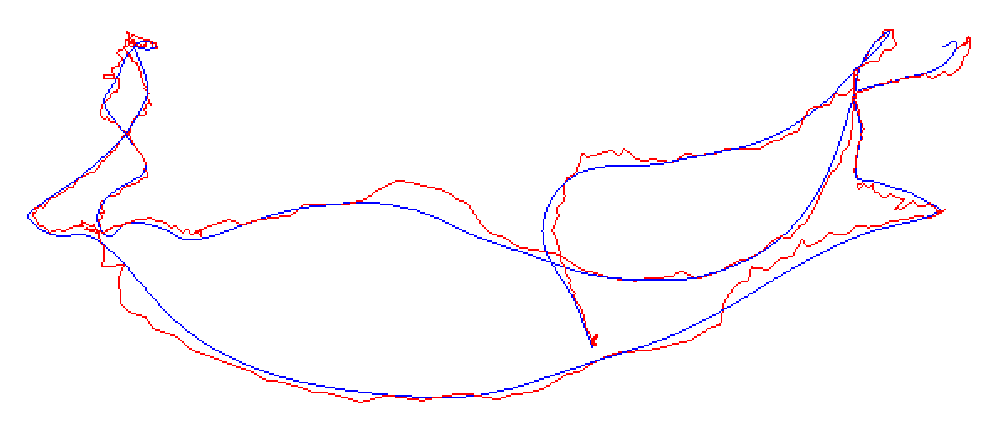
\includegraphics[width=1.0\textwidth]{lieGroup/trajectory-compare.pdf}
    \caption{Calculates the error between the estimated trajectory and the real trajectory. }
    \label{fig:trajectory-compare}
\end{figure}

\section{Similar Transform Group and Its Lie Algebra}
Finally, we would like to mention the similar transform group $\mathrm{Sim}(3)$ used in monocular vision, and the corresponding Lie algebra $\mathfrak{sim}(3)$. If you are only interested in stereo or RGB-D SLAM, you can skip this section.

We have already introduced the concept of scale ambiguity. If $\mathrm{SE}(3)$ is used in the monocular SLAM to represent the pose, then the scale in the entire SLAM process will change due to scale uncertainty and scale drift, which is what $\mathrm{SE}(3) $ not reflects. Therefore, in the case of monocular SLAM, we generally express the scale factor explicitly. In mathematical terms, for the point $\mathbf{p}$ in space, a \textit{similar transformation} is passed in the camera coordinate system instead of the Euclidean transformation:
\begin{equation}
\mathbf{p}' = \left[ {\begin{array}{*{20}{c}}
    {s\mathbf{R}}&\mathbf{t}\\
    {{\mathbf{0}^T}}&1
    \end{array}} \right] \mathbf{p}
= s\mathbf{R} \mathbf{p} + \mathbf{t}.
\end{equation}
In the similarity transformation, we express the scale as $s$. It also acts on top of the three coordinates of $\mathbf{p}$ and scales $\mathbf{p}$ once. Similar to $\mathrm{SO}(3)$, $\mathrm{SE}(3)$, the similarity transform also forms a group on matrix multiplication, called the similarity transform group $\mathrm{Sim}(3)$:
\begin{equation}
\mathrm{Sim}(3) = \left\{ { \mathbf{S} = \left[ {\begin{array}{*{20}{c}}
        {s\mathbf{R}}& \mathbf{t}\\
        {{\mathbf{0}^T}}&1
        \end{array}} \right] \in {\mathbb{R}^{4 \times 4}}} \right\}.
\end{equation}

Similarly, $\mathrm{Sim}(3)$ also has corresponding Lie algebra, exponential mapping, logarithmic mapping, and so on. The Lie algebra $\mathfrak{sim}(3)$ element is a 7-dimensional vector $\boldsymbol{\zeta}$. Its first 6 dimensions are the same as $\mathfrak{se}(3)$, followed by a $\sigma$ to denote the scale.

\begin{equation}
\mathfrak{sim} \left( 3 \right) = \left\{ { \boldsymbol{\zeta} | \boldsymbol{\zeta} = \left[ \begin{array}{l}
    \boldsymbol{\rho} \\
    \boldsymbol{\phi} \\
    \sigma
    \end{array} \right] \in { \mathbb{R}^7},{ \boldsymbol{\zeta} ^ \wedge } = \left[ {\begin{array}{*{20}{c}}
        {\sigma \mathbf{I} + {\boldsymbol{\phi} ^ \wedge }}&\boldsymbol{\rho} \\
        {{\mathbf{0}^T}}&0
        \end{array}} \right] \in {\mathbb{R}^{4 \times 4}}} \right\}.
\end{equation}

It has an additional $\sigma$ compared with $\mathfrak{se}(3)$. The $\mathrm{Sim}(3)$ and $\mathfrak{sim}(3)$ are still associated with exponential maps and logarithm maps. The exponential mapping is:

\begin{equation}
\exp \left( {{ \boldsymbol{\zeta} ^ \wedge }} \right) = \left[ {\begin{array}{*{20}{c}}
    {{\mathrm{e}^\sigma }\exp \left( {{ \boldsymbol{\phi} ^ \wedge }} \right)}&{ \mathbf{J}_s \boldsymbol{\rho} }\\
    {{\mathbf{0}^T}}&1
    \end{array}} \right],
\end{equation}
where $\mathbf{J}_s$ is:
\begin{align*}
%\begin{array}{ll}
{ \mathbf{J}_s} =& \frac{{{\mathrm{e}^\sigma } - 1}}{\sigma } \mathbf{I} + \frac{ \sigma {{\mathrm{e} ^\sigma }\sin \theta + \left( {1 - {\mathrm{e}^\sigma }\cos \theta } \right)\theta }}{{{\sigma ^2} + {\theta ^ 2}}}{\mathbf{a}^ \wedge }\\
&+ \left( {\frac{{{\mathrm{e}^\sigma } - 1}}{\sigma } - \frac{{\left( {{\mathrm{e}^\sigma }\cos \theta - 1} \right)\sigma + ({\mathrm{e}^\sigma }\sin \theta )\theta }}{{{\sigma ^2} + {\theta ^2}}}} \right ){\mathbf{a}^ \wedge }{\mathbf{a}^ \wedge }.
%\end{array}
\end{align*}

Through exponential mapping, we can find the relationship between Lie algebra and Lie group. For the Lie algebra $\boldsymbol{\zeta}$, its correspondence with the Lie group is:
\begin{equation}
s=\mathrm{e}^\sigma, \; \mathbf{R} = \exp( \boldsymbol{\phi} ^\wedge), \; \mathbf{t} = \mathbf{J}_s \boldsymbol{ \rho}.
\end{equation}

The rotation is consistent with $\mathrm{SO}(3)$. In the translation part, we need to multiply a Jacobian $\boldsymbol{\mathcal{J}}$ in $\mathfrak{se}(3)$, and the similarly transformed Jacobi is more complicated. For the scale factor, you can see that $s$ in the Lie group is the exponential function of $\sigma$ in the Lie algebra.

The BCH approximation of $\mathrm{Sim}(3)$ is similar to $\mathrm{SE}(3)$. We can discuss a derivative of $\mathbf{S}$ after a similar transformation of $\mathbf{S} \mathbf{p}$ relative to $\mathbf{S}$. Similarly, there are two ways of the differential model and perturbation model, and the perturbation model is the simpler one. We omit the derivation process and directly give the results of the perturbation model. Let $\mathbf{S} \mathbf{p}$ a small perturbation $\exp( \boldsymbol{\zeta} ^\wedge )$ on the left and ask for $\mathbf{S} \mathbf{p}$ The derivative of the disturbance. Since $\mathbf{S} \mathbf{p}$ is a 4-dimensional homogeneous coordinate, $\boldsymbol{\zeta}$ is a 7-dimensional vector, which should have $4 \times 7$ Jacobian. For convenience, remember the first three-dimensional composition vector $\mathbf{q}$ of $\mathbf{Sp}$, then:

\begin{equation}
\frac{{\partial \mathbf{Sp}}}{{\partial \boldsymbol{\zeta} }} = \left[ {\begin{array}{*{20}{c}}
    \mathbf{I} &{ - {\mathbf{q}^ \wedge }}& \mathbf{q} \\
    {{\mathbf{0}^T}} & {{ \mathbf{0}^T}}&0
    \end{array}} \right].
\end{equation}

We will end here about the contents of $\mathrm{Sim}(3)$. For more detailed information on $\mathrm{Sim}(3)$, please refer to the literature~\cite{Strasdat2012a}.

\section{Summary}
This lecture introduces Lie group $\mathrm{SO}(3)$ and $\mathrm{SE}(3)$, and their corresponding Lie algebras $\mathfrak{so}(3)$ and $\mathfrak{se }(3)$. We introduce the expression and transformation of poses on them, and then through the linear approximation of BCH, we can perturb and predict the pose. This lays the theoretical foundation for optimizing the pose afterward because we need to adjust the estimate of a certain pose frequently to reduce the corresponding error. Only after we have figured out how to adjust and update the pose can we continue to the next step.

The content of this lecture may be more theoretical. After all, it is not as good as computer vision. Compared to the mathematics textbooks that explain Lie group Lie algebra, since we only care about practical content, the process is very streamlined, and the speed is relatively fast. The reader must understand the content of this lecture, which is the basis for solving many subsequent problems, especially the pose estimation part.

It should be mentioned that in addition to the Lie algebra, the rotation can also be expressed by quaternion, Euler angle, etc., but the subsequent processing is troublesome. In practice, you can also use $\mathrm{SO}(3)$ plus a translation instead of $\mathrm{SE}(3)$ to avoid some Jacobian calculations.

\section*{Exercises}
\begin{enumerate}
    \item Verify $\mathrm{SO}(3)$, $\mathrm{SE}(3)$, and $\mathrm{Sim}(3)$ are groups on matrix multiplication.
    \item Verify that $( \mathbb{R}^3, \mathbb{R}, \times )$ constitutes a Lie algebra.
    \item Verify that $\mathfrak{so}(3)$ and $\mathfrak{se}(3)$ satisfy the requirements of Lie algebra.
    \item Verify the properties (4.20) and (4.21).
    \item Show that: \[
    \mathbf{R} \mathbf{p}^\wedge \mathbf{R}^T = (\mathbf{Rp})^\wedge .\]
    \item Show that: \[
    \mathbf{R} \exp( \mathbf{p}^\wedge) \mathbf{R}^T = \exp( (\mathbf{Rp})^\wedge ).\] This is called the \textit{adjoint} property on $\mathrm{SO}(3)$. Similarly, there is an adjoint property on $\mathrm{SE}(3)$:
    \begin{equation}
    \mathbf{T} \exp(\boldsymbol{\xi}^\wedge)\mathbf{T}^{-1} = \exp \left( \left( \mathrm{Ad}(\mathbf{T}) \boldsymbol{\xi} \right) ^\wedge \right),
    \end{equation}
    where
    \begin{equation}
    \label{eq:adjSE3}
    \mathrm{Ad} ( \mathbf{T} ) = \left[ {\begin{array}{*{20}{c}}
        \mathbf{R} &{{ \mathbf{t} ^ \wedge } \mathbf{R} }\\
        \mathbf{0} & \mathbf{R}
        \end{array}} \right].
    \end{equation}
    \item Follow the derivation of the left perturbation and derives the derivatives of $\mathrm{SO}(3)$ and $\mathrm{SE}(3)$ under the right perturbation.
    \item Search how CMake's \textit{find\_package} works. What optional parameters does it have? What are the prerequisites for CMake to find a library?
\end{enumerate}
